% ---------------------------------------------------------
\chapter{Big Picture}
\label{chap:method}
% ---------------------------------------------------------
This chaper super intro because importantst chapter


\section{Process}

Goal: we need software to test the performance 

Defining: of configuration options of the software
workload of the software

profile software execution \ref{perf_measure}
choose appropriate sampling strategie
repeate execution number sample times

because software runs on real hardware measurements might be biased
extract execution bias (external mesurement impact)

if bias is acceptable use data to learm variability model of software 

if it is acceptable calculate model for each function (WHY?)
showing influences of configuration options to each function

Visualisation plugin eclipse to mark possible hot-spots direct in IDE

Flame Graph as overview distribution of functions



Our Workflow:

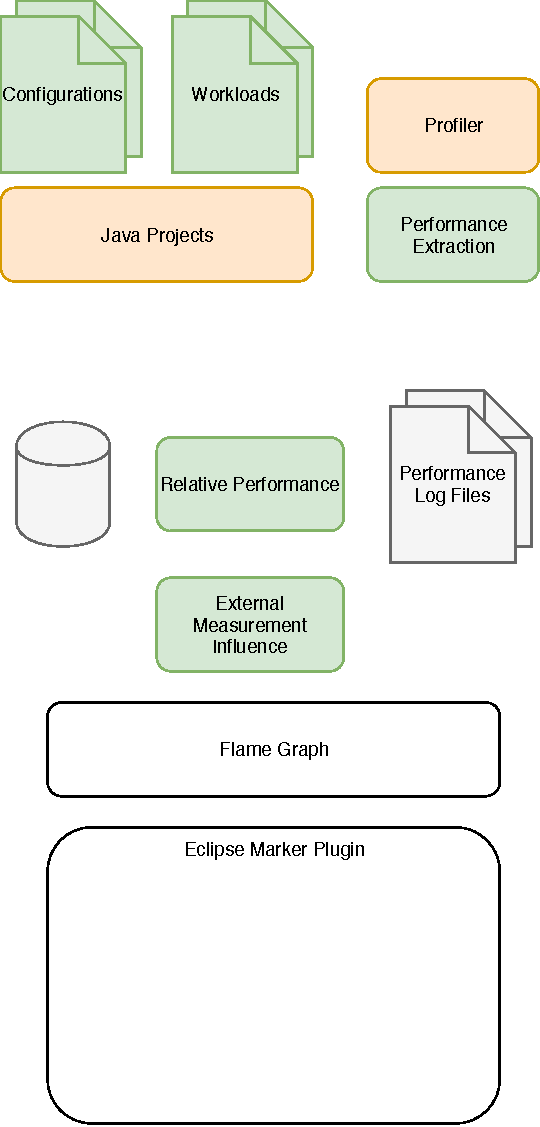
\includegraphics[width=0.6\textwidth]{images/Workflow}

\section{Case Studies}
\label{case_studies}

Eingrenzung auf Java software because, widespread, popular, often used, runs on billions of devices

% 3 Java projects 
% 3 different kinds of projects to depict variety
% Configurable, Workload of projects to manage execution time and to validate results of projects with different workloads
% different configuration space 
% different ammount of configuration options
% 

\subsection{Catena}

 Project description
% Project size in Classes and Functions
% Project properties (SPL Model)
% Features explained
% Workload

\subsection{H2}

Project description
% Project size in Classes and Functions
% Project properties (SPL Model)
% Features explained
% Workload

\subsection{Sunflow}

Project description
% Project size in Classes and Functions
% Project properties (SPL Model)
% Features explained
% Workload

\section{Sampling}
\label{perf_measure_sampling}

Why sampling?
Configuration space 
Course of high dim spaces
Random Sampling

\subsection{Binary Sampling}

\subsubsection{Option-Wise}

\subsubsection{Negative-Option-Wise}

\subsubsection{t-Wise}

\subsubsection{Binary-Random}


% Why random ... other paper.

\subsection{Numeric Sampling}

\subsubsection{One Factor at a Time}

\subsubsection{Central Composite}

\subsubsection{Placket-Burman Design}

% other strats
% Distance computation

\section{Monitoring/Profiling}
pitfalls
strategies 
solutins
expected outcome
